\section{Preliminary experiments}
Here we describe one numerical simulation from each code to give a
qualitative picture of disc evolution. 
%In the next section, we analyse
%2D simulations in more detail and explore parameter space with
%improved resolution runs.   

In these simulations we subject the disc to random perturbations in
cylindrical velocity,
\begin{align}\label{randpert}
  \frac{\delta v_R}{c_s} = \frac{\delta}{M}\times T(R) \sum_{m=1}^M\cos{m\phi},
\end{align}
where $\delta$ is an amplitude and 
\begin{align}
  T(R) =
  \exp{\left[-\frac{1}{2}\left(\frac{R-\overline{R}_d}{\Delta
          R_d}\right)^2\right]}, 
\end{align}
where $\overline{R}_d = (R_{d1}+R_{d2})/2$ and $\Delta R_d =
(R_{d2}-R_{d1})/2$. 
\subsection{2D run}\label{fargo_fiducial}
We consider a disc size $[R_\mathrm{min}, R_\mathrm{max}] =
[0.4,10]R_0$. This gives a total disc mass $M_{d}=0.086M_*$, and the
mass within $R\in[R_{d1},R_{d2}]$ is $0.049M_*$. 
We use a resolution of $N_R\times N_\phi = 1024\times 2048$ or
about $16$ grids per $H$, and adopt $\epsilon_g=10^{-4}H$ for the 
self-gravity softening length\footnote{In 2D self-gravity, $\epsilon_g$ also
  approximates for the vertical disc thickness, so a more appropriate
  value would be $\epsilon_g\sim H$ \citep{muller12}. However, because
  $\epsilon_g\propto R$ is needed in FARGO, the Poisson kernel
  (Eq. \ref{2d_grav}) is no longer symmetric in $(R,R^\prime)$. We
  choose a small  
  $\epsilon_g$ in favour of angular momentum conservation, keeping in
  mind that the strength of self-gravity will be over-estimated.}.
Perturbations are set initially with $M=10$ and
$\delta\in[-10^{-3},10^{-3}]$ chosen randomly but does not depend
on $\phi$. 

%set $M=10$ for random perturbations (Eq. \ref{randpert}). 

Snapshots from the disc evolution are shown in Fig. \ref{fargo_2d} in
terms of the non-axisymmetric surface density. At early times
$t\lesssim100P_0$ the disc is dominated by low-amplitude high-$m$
perturbations centred in the dead zone. Eventually a $m=1$ spiral 
grows and dominates inside the dead zone.  

Fig. \ref{fargo_2d_angmom} compares the disc angular momenta
evolution, most of which is contained in the $m=0$ and $m=1$ modes. 
The $m=1$ spiral has an associated negative angular
momentum. Its growth is correlated with an increase in the axisymmetric
component of angular momentum, such that $\Delta J_0 \sim - \Delta
J_1$. Note that FARGO does not explicitly conserve angular
momentum. In addition, there may be an angular momentum flux due to
self-gravity across disc boundaries since our domain size is finite. 
Nevertheless, we find the total angular momentum is conserved to 
$|\Delta J/J|= O(10^{-6})$, and is much smaller in magnitude than the change in the
angular momenta components, $|\Delta J_{0,1}/J|> O(10^{-5})$. 
Fig. \ref{fargo_2d_angmom} then indicates a transfer of 
angular momentum from the $m=1$ spiral to the background disc. 

\begin{figure}
  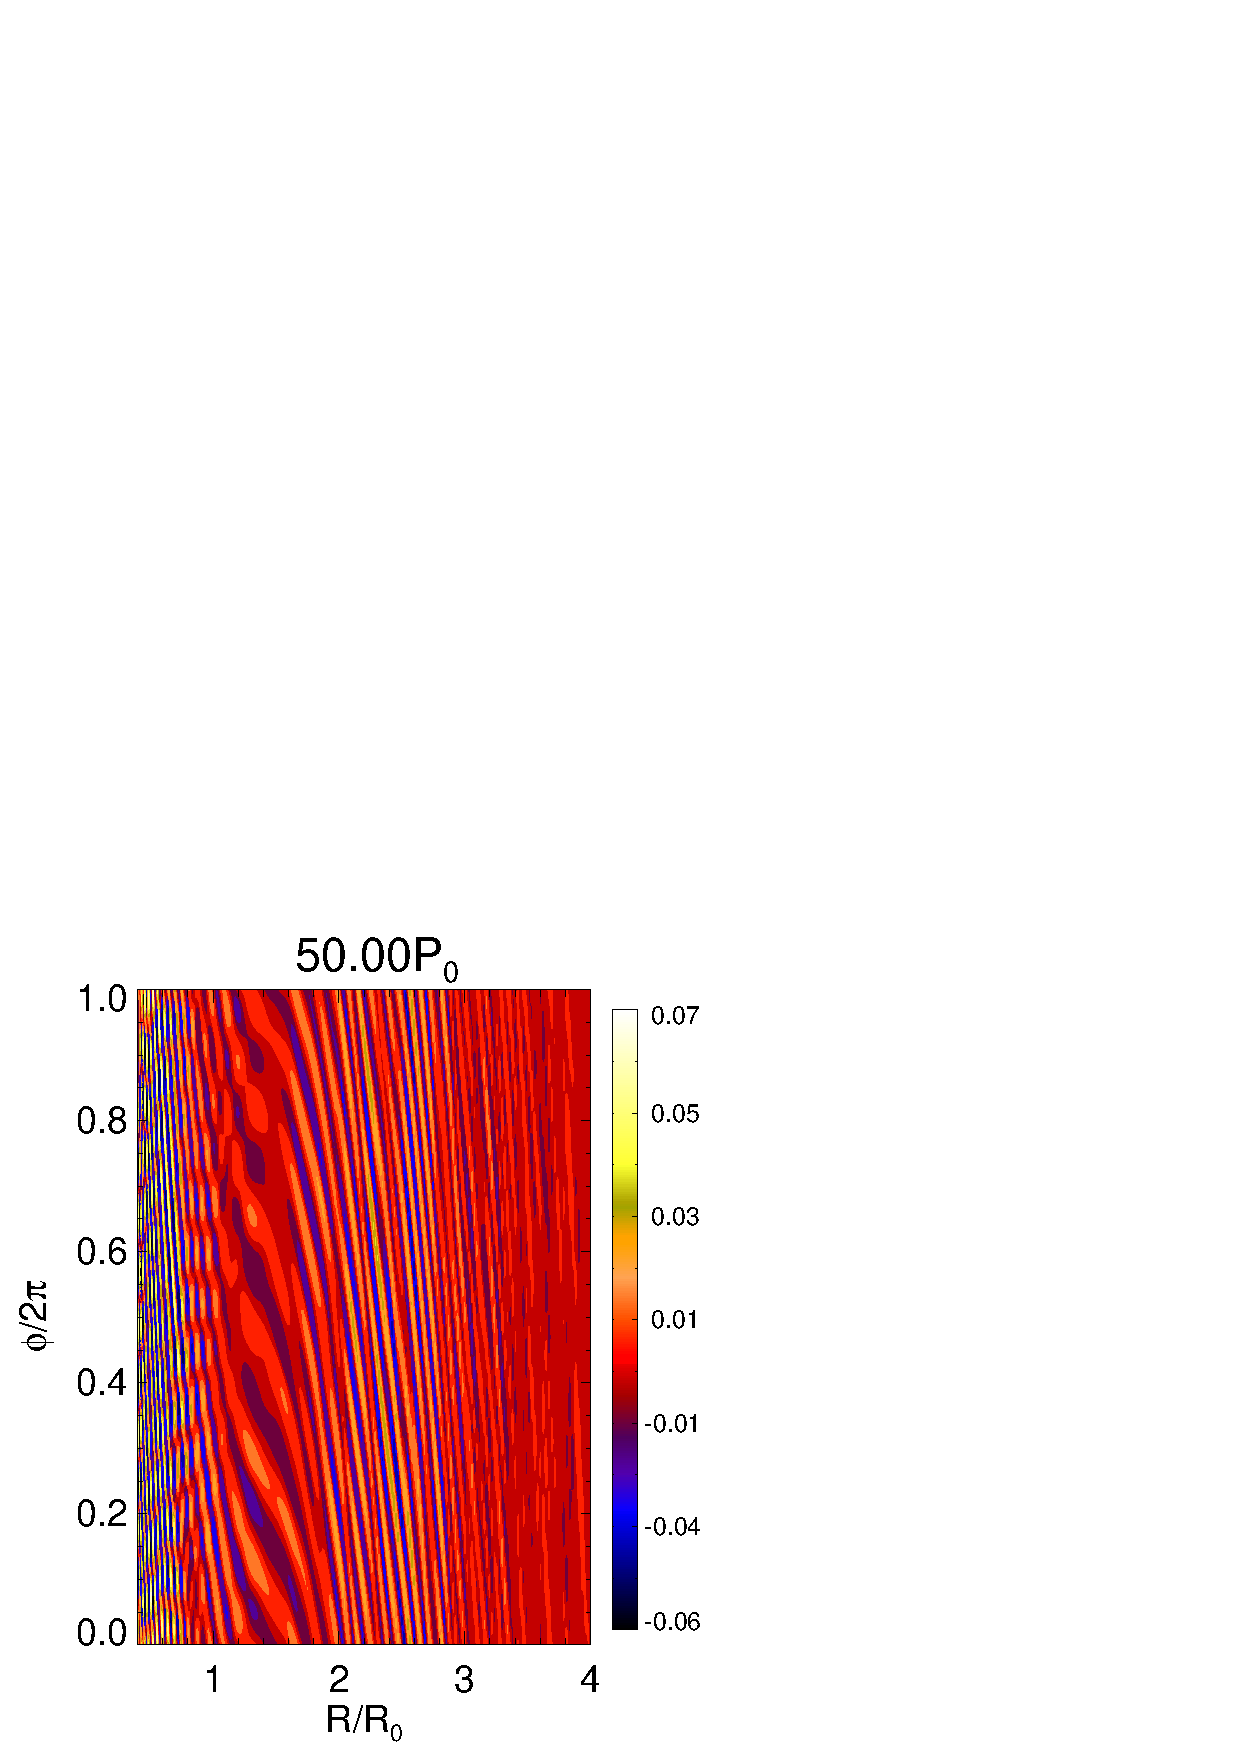
\includegraphics[scale=0.27]{figures/polarxy_dens050}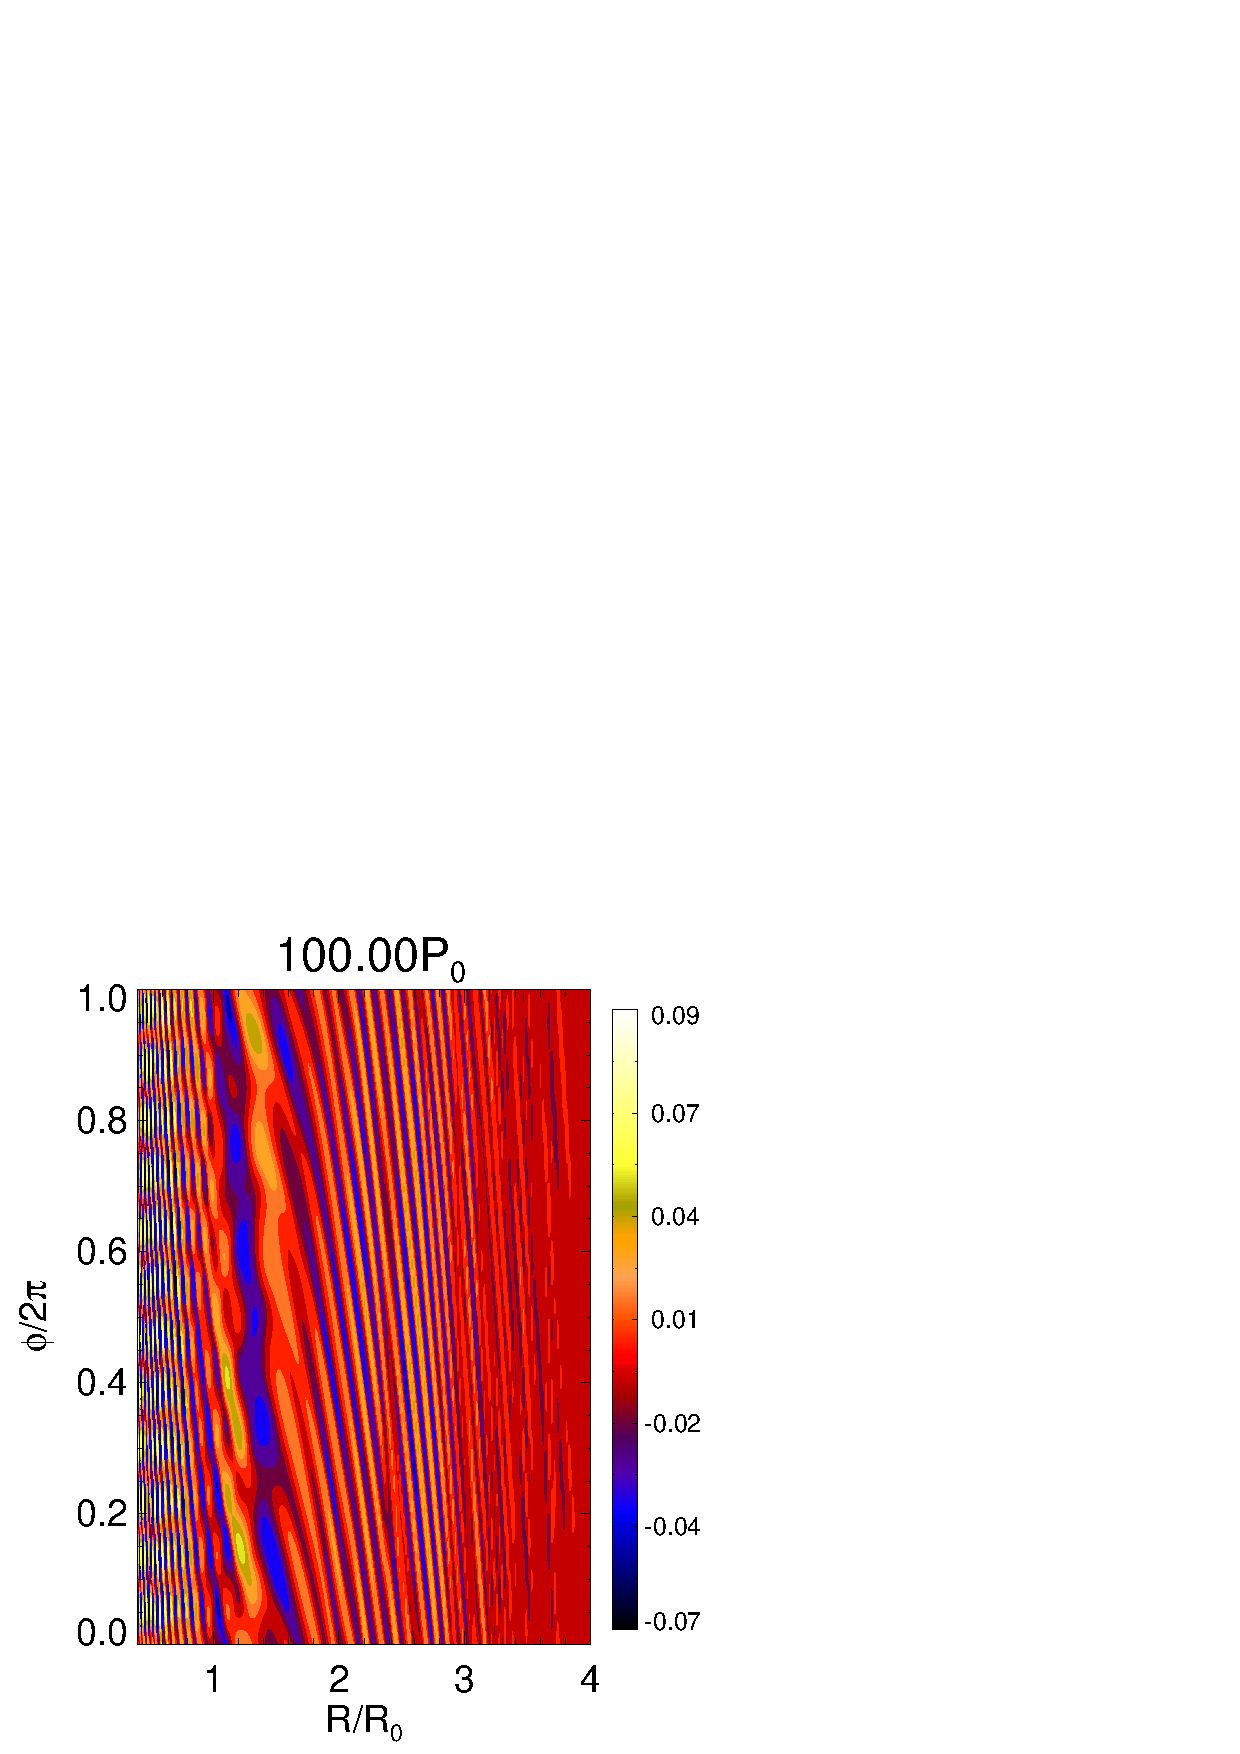
\includegraphics[scale=0.27,clip=true,trim=2.26cm 
  0cm 0cm
  0cm]{figures/polarxy_dens100}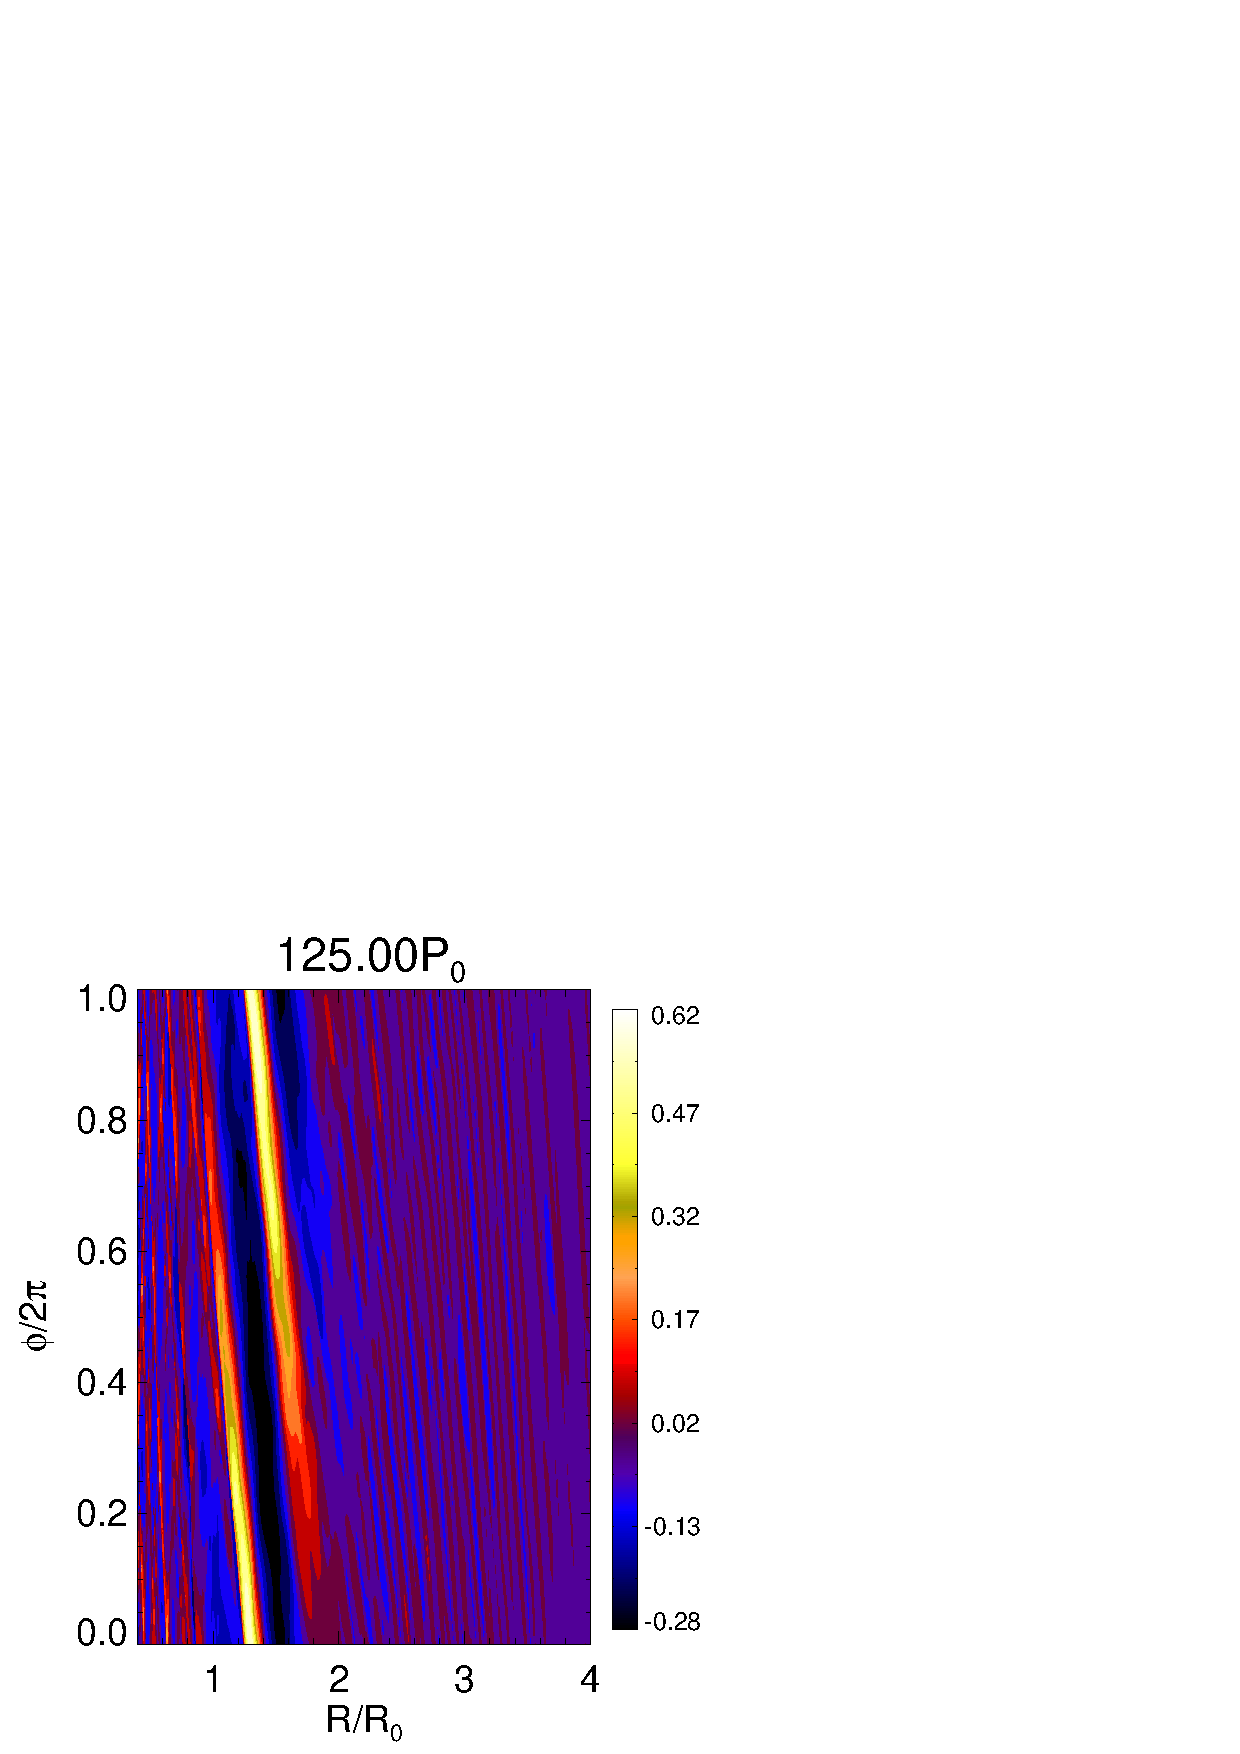
\includegraphics[scale=0.27,clip=true,trim=2.26cm
  0cm 0cm 0cm]{figures/polarxy_dens125} 
  \caption{Preliminary FARGO 2D simulation (\S\ref{fargo_fiducial}),
    showing the evolution of the non-axisymmetric surface density
    $\Delta\Sigma$. Note that the disc extends to $R=10R_0$, but only
    the inner part is shown for clarity. \label{fargo_2d}} 
\end{figure}

\begin{figure}
  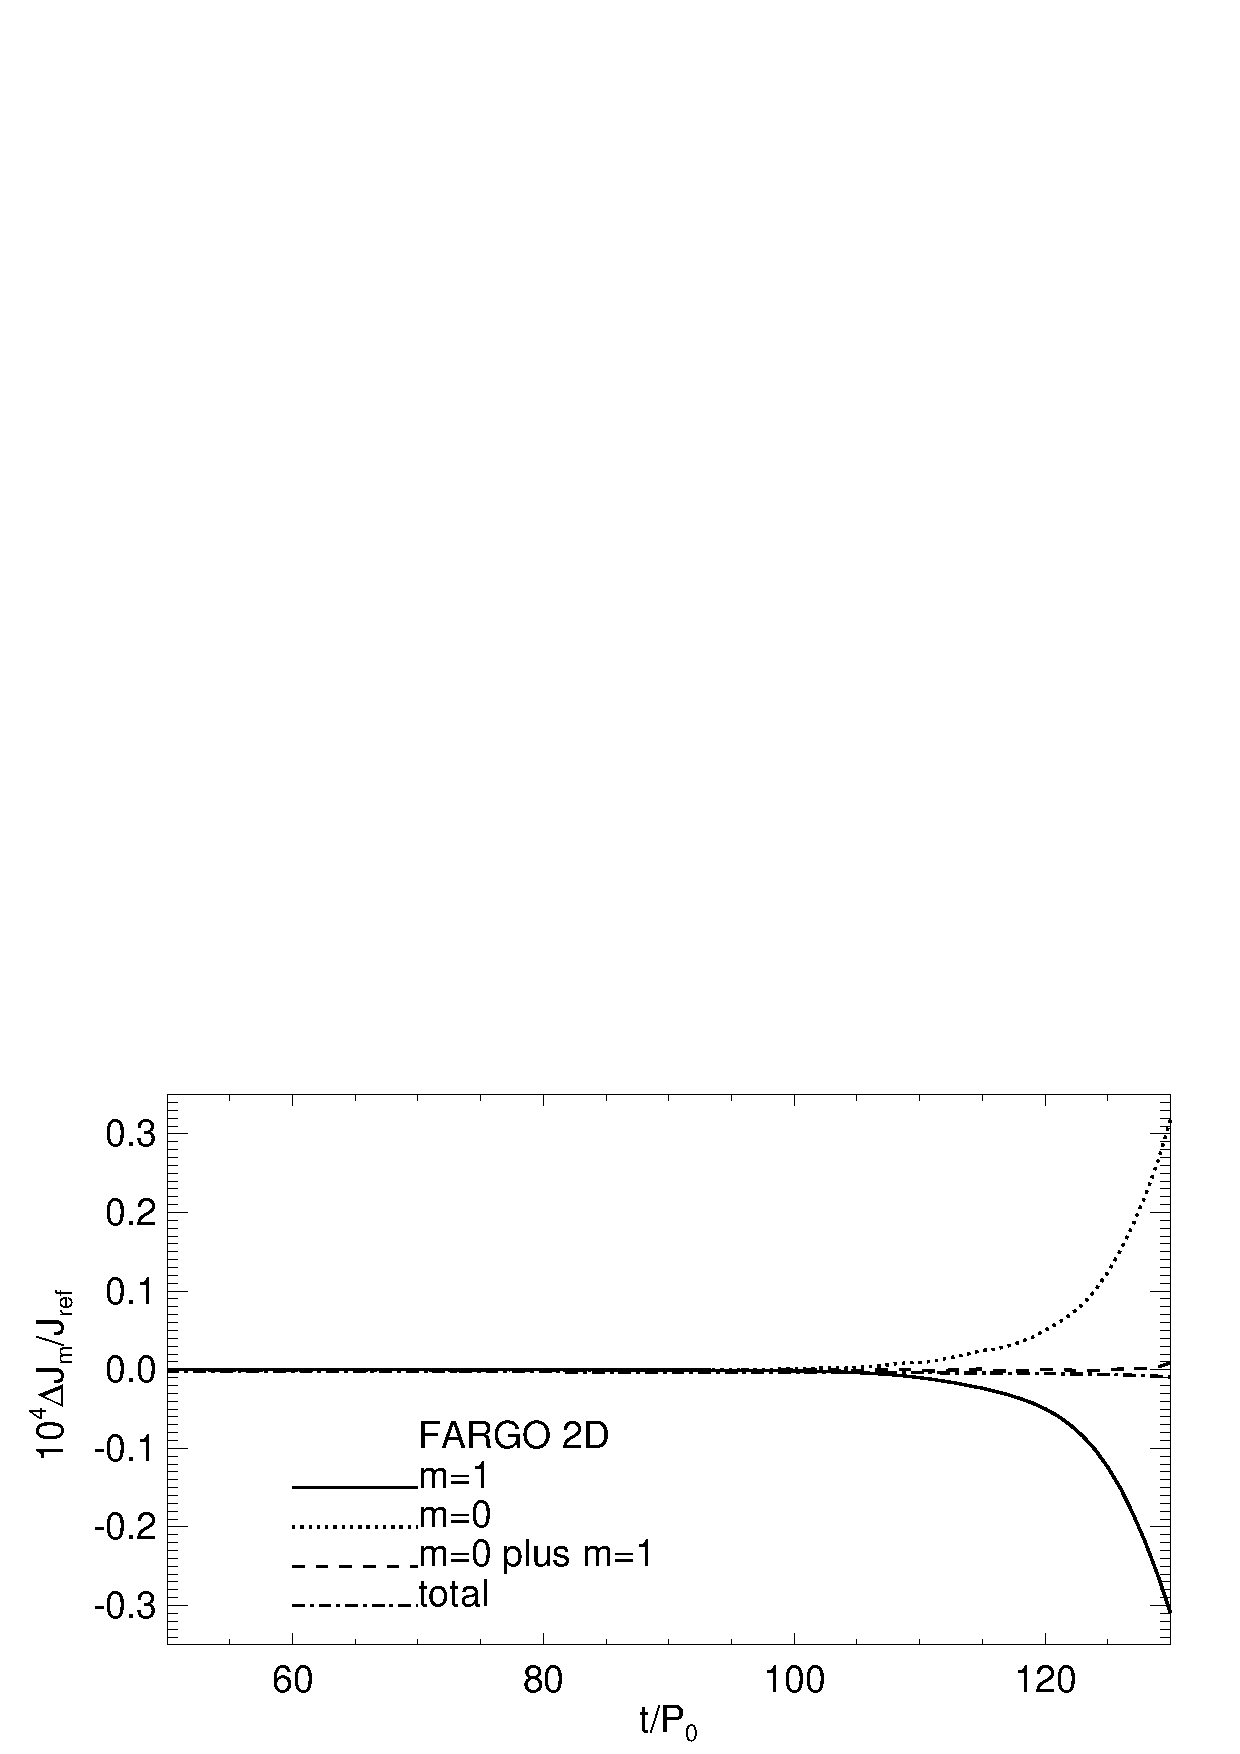
\includegraphics[width=\linewidth]{figures/nonaxi_evol_ang_fargo}
  \caption{Evolution of angular momentum components in the FARGO
     simulation show in Fig. \ref{fargo_2d}. The perturbation
    relative to $t=0$ is shown in units of the initial total angular
    momentum $J_\mathrm{ref}$.\label{fargo_2d_angmom}} 
\end{figure}

\subsection{3D runs}
The 3D disc has radial size 
$[r_\mathrm{min},r_\mathrm{max}]=[0.4,10]R_0$ and vertical extent
$n_H=2$ scale-heights. The resolution is $N_r\times N_\theta\times
N_\phi=256\times32\times256$. Because of the much reduced resolution
compared to 2D, we use a smooth perturbation by setting
$\delta = 10^{-3}$ and $M=1$. This corresponds to a single $m=1$
spiral in the dead zone, which was found to dominate the 2D
simulation. 

Our 3D discs are initialised in approximate equilibrium only, so we
first evolve the disc without perturbations using  
$(\lmax,\mmax)=(32,0)$ up to $t=10P_0$, during which 
meridional velocities are damped out. We then restart the simulation
with the above perturbation and $(\lmax,\mmax)=(32,32)$. 

Snapshots at the end of the simulations are shown in
Fig. \ref{3d_prelim} for both ZEUS-MP and PLUTO. We again
find the dead zone eventually dominated by an $m=1$ spiral. Note that
the amplitude of the spiral is smaller than the 2D case above,
possibily due to lower resolution and/or 3D self-gravity being weaker
than that in 2D. 

\begin{figure}
  \begin{center}
    \subfigure[ZEUS-MP]{
      \includegraphics[scale=0.33]{figures/polarxy_dens015_zeus}
    }
    \subfigure[PLUTO]{
      \includegraphics[scale=0.33]{figures/polarxy_dens015_zeus}
    }
  \end{center}
  \caption{Preliminary 3D simulations using the (a) ZEUS-MP and (b)
    PLUTO. The non-axisymmetric midplane density at the end of the run
    is shown. Here $\psi \equiv \pi/2 - \theta$ is the angular height
    from the midplane.\label{3d_prelim}}   
\end{figure}


Fig. \ref{3d_prelim_angmom} shows the angular momentum evolution in
the 3D runs. ZEUS-MP does not conserve angular momentum very well, but
the variation $|\Delta J/J|< O(10^{-5})$ is not significant compared
to the individual components $|\Delta J_{0,1}/J|\sim
6\times10^{-5}$. We found high-$m$ structures to develop near the
inner boundary, which may have contributed to this error. It
is clear, however, that the growth of negative angluar momentum in
$m=1$ is accompanied by an increase in the background angular
momentum. 

\begin{figure}
  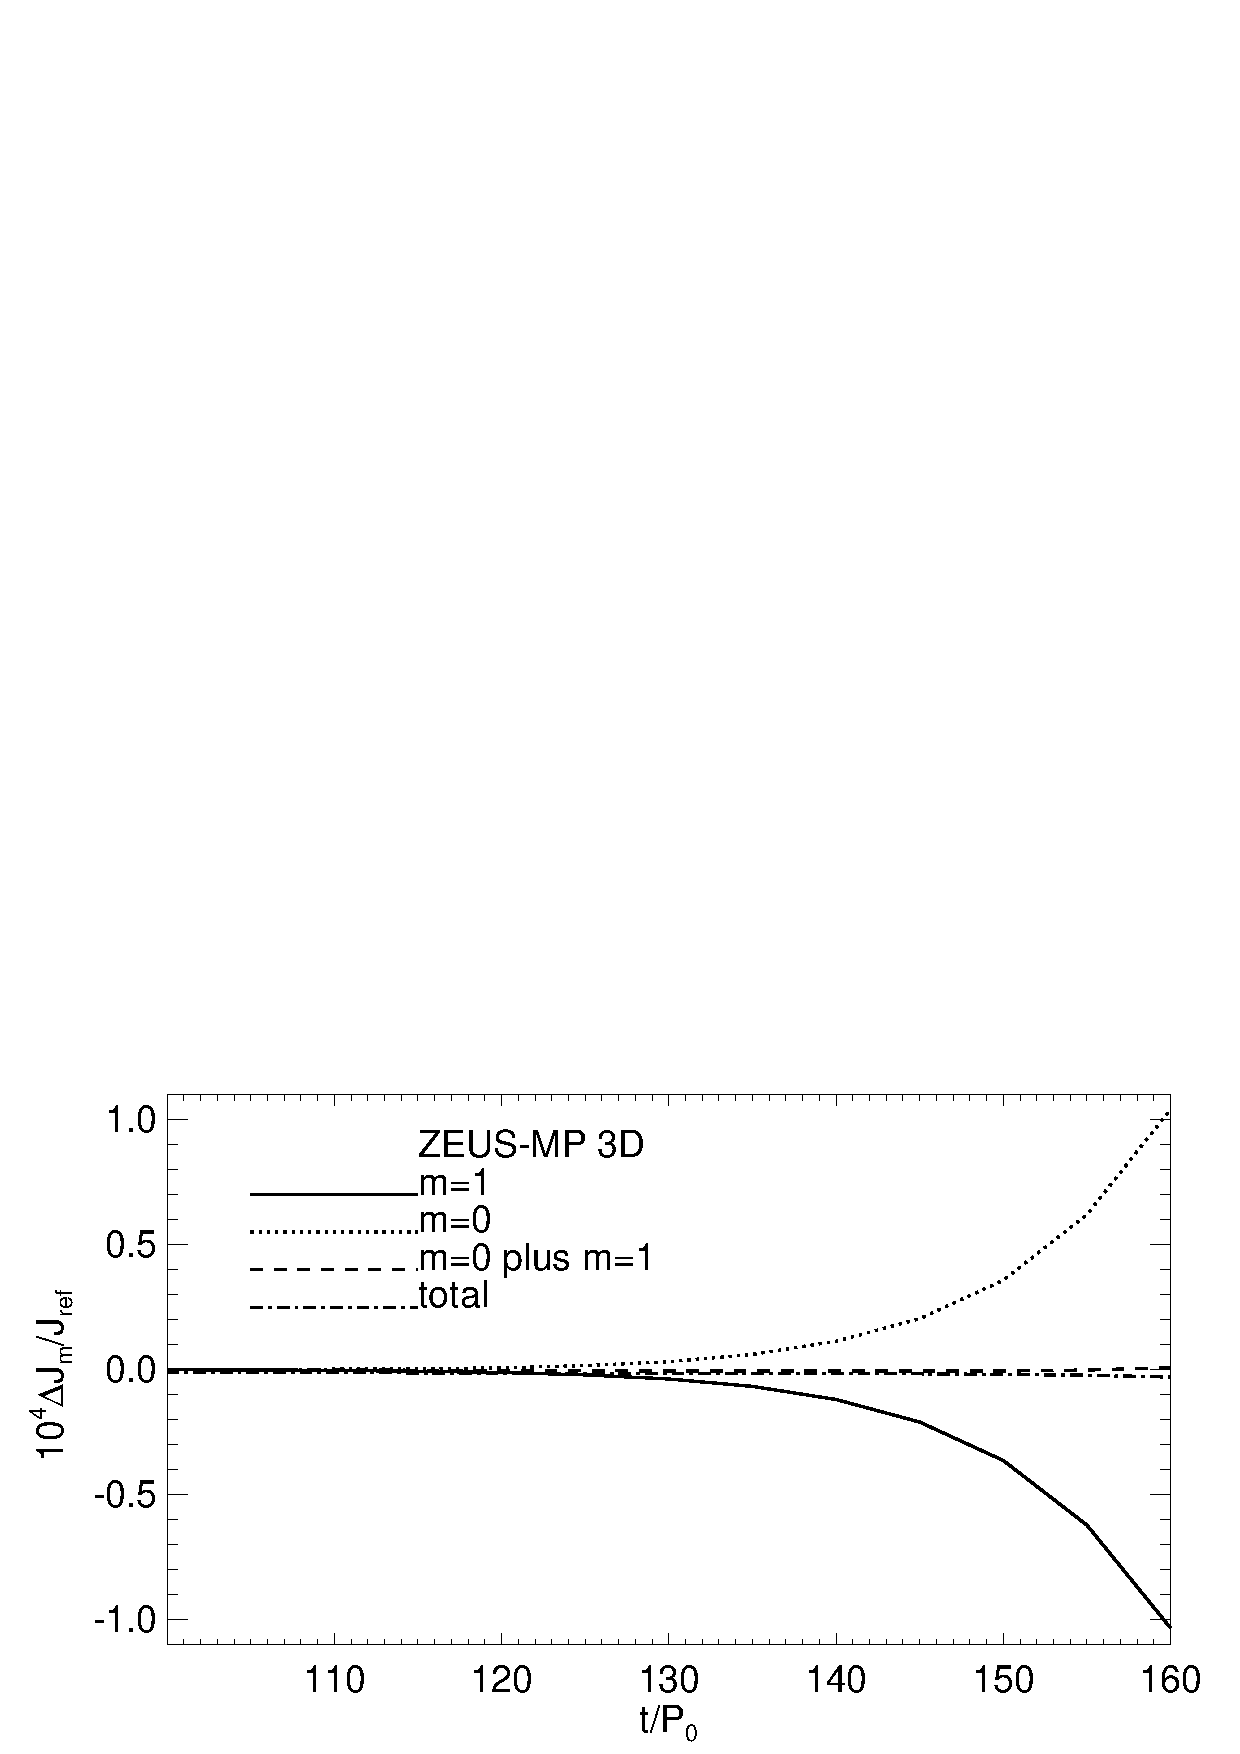
\includegraphics[scale=0.41,clip=true,trim=0cm 1.75cm 0cm 0cm]{figures/nonaxi_evol_ang_zeus}
  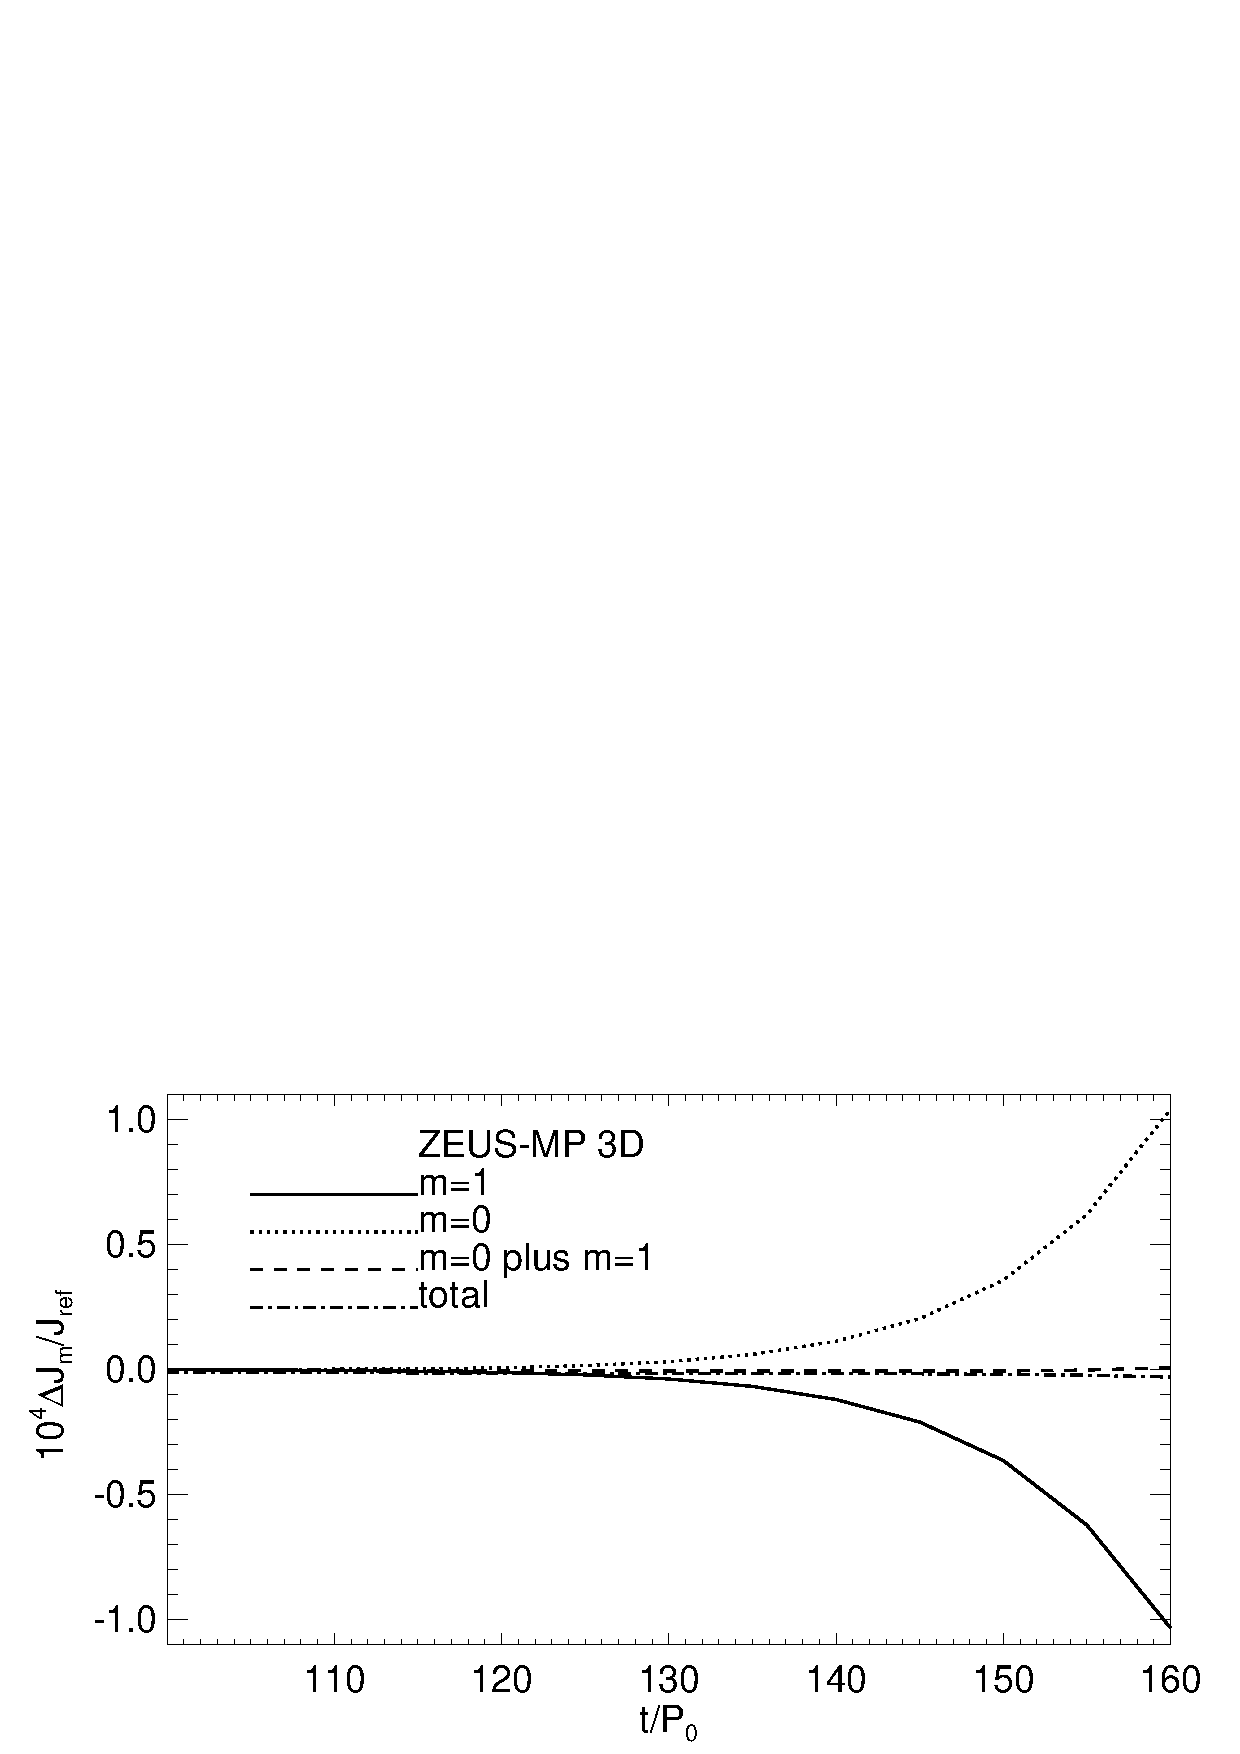
\includegraphics[scale=0.41]{figures/nonaxi_evol_ang_zeus}
  \caption{Evolution of angular momentum components in the 3D 
    simulations show in Fig. \ref{3d_prelim}. The perturbation
    relative to $t=10P_0$ is shown in units of the initial total
    angular momentum $J_\mathrm{ref}$.\label{3d_prelim_angmom}} 
\end{figure}   

\section{Global one-arm spirals in structured discs}

\subsection{Properties of the $m=1$ dead zone spiral}

%\subsection{Three-dimensional structure}

%\section{Additional simulations}
%survery